\chapter{Special Topics in Physics}\label{ap:spec_phys}
Section~\Ref{sec:isohyper} follows Chapter~9 of 
Thomson~\cite{thomson_modern_2013}. 
Section~\Ref{sec:ssb} follows Section~11.1 of Peskin and 
Schroeder~\cite{peskin_introduction_1995}.
Sections~\Ref{sec:cscont} and 
\Ref{sec:cslat} follow Chapter 7 of Gattringer and 
Lang~\cite{gattringer_quantum_2010}. 

\section{Isospin and hypercharge}\label{sec:isohyper}
\index{hypercharge}\index{isospin}
In quantum mechanics you learn that spin is a quantum number of
charged particles. For example the electron is a spin-1/2 particle. The
$z$-component $S_3$ of the spin operator $S$ commutes with the Hamiltonian, and
you learn that the eigenvectors of $S_3$ are the +1/2 and -1/2 states. You also
learn that the components of $S$ are related to the Pauli matrices by
\begin{equation}
  S_i=\frac{\hbar}{2}\sigma_i.
\end{equation}

Early on in nuclear physics, scientists noticed that the proton and neutron had
about the same mass, and that the nuclear force between two nucleons (i.e.
protons or neutrons) was approximately charge independent. Therefore Heisenberg
suggested that protons and neutrons were two states of a single particle (the
nucleon) just as there are spin-up and spin-down states of a spin-1/2
particle.
The quantum number corresponding to this property is called {\it isospin}.
Using this idea, the proton and neutron form an isospin doublet with total
isospin $I=1/2$ and $z$-component $I_3=\pm1/2$. Thus the Pauli matrices also
give a suitable representation of the isospin operator, and we write
\begin{equation}
  I^2=\sum\limits_{i=1}^3 I_i^2, \qquad I_i=\frac{1}{2}\sigma_i.
\end{equation}
I know this is sloppy, but I want to leave it to the reader to determine from
context whether $I$ represents the operator or the eigenvalue. 

The concept of isospin can be extended in the same way to quarks. 
In the simplest case we have $N_f=2$ and consider the lightest quarks
$u$ and $d$. The $\SU(2)$ isospin symmetry is only approximate because 
the $u$ and $d$ quarks have slightly different masses. The isospin 
doublet then has a $u$ component and a $d$ component. Generally with
$N_f$ flavors of fermion, the symmetry group is $\SU(N_f)$ and we
form $N_f$ component multiplets in flavor space, one component per flavor.

Let's introduce the $s$ quark and do the $N_f=3$ case.
Using the Pauli matrices and the fact that $\SU(3)$ has 8 generators, you can
figure out what the Gell-Mann matrices are. We will say that $u$, $d$, and $s$
are eigenvectors of isospin and write
\begin{equation}
  u=\colvec{3}{1}{0}{0}, \qquad
  d=\colvec{3}{0}{1}{0}, \qquad
  s=\colvec{3}{0}{0}{1}.
\end{equation}
Then $u$ and $d$ span a 2D subspace of flavor space, so from the earlier
discussion we should know that the generators of $\SU(2)$ are contained in the
generators of $\SU(3)$. Hence
\begin{equation}
  \lambda_1=\left(\begin{array}{ccc}
            0 & 1 &  \\
            1 & 0 &  \\
              &   & 0
            \end{array}\right), \qquad
  \lambda_2=\left(\begin{array}{ccc}
            0 & -i &  \\
            i & 0  &  \\
              &    & 0
            \end{array}\right), \qquad
  \lambda_3=\left(\begin{array}{ccc}
            1 & 0  &  \\
            0 & -1 &  \\
              &    & 0
            \end{array}\right).
\end{equation}
But there's nothing special about $u$ and $d$; $u$ and $s$ will similarly form
a subspace, and so will $d$ and $s$. In both cases, we will use the Pauli
matrices as generators. We can similarly write
\begin{equation}
  \lambda_4=\left(\begin{array}{ccc}
            0 &   & 1\\
              & 0 &  \\
            1 &   & 0
            \end{array}\right), \qquad
  \lambda_5=\left(\begin{array}{ccc}
            0 &    & -i \\
              & 0  &    \\
            i &    & 0
            \end{array}\right), \qquad
  \lambda_X=\left(\begin{array}{ccc}
            1 &    & 0 \\
              & 0  &   \\
            0 &    & -1
            \end{array}\right),
\end{equation}
\begin{equation}
  \lambda_6=\left(\begin{array}{ccc}
            0 &   &  \\
              & 0 & 1\\
              & 1 & 0
            \end{array}\right), \qquad
  \lambda_7=\left(\begin{array}{ccc}
            0 &    &   \\
              & 0  & -i\\
              & i  & 0
            \end{array}\right), \qquad
  \lambda_Y=\left(\begin{array}{ccc}
           0  &    &  \\
              & 1  & 0\\
              & 0  & -1 
            \end{array}\right).
\end{equation}
Finally note the fact that there are only 8 linearly independent generators, so
two of these matrices should be linearly dependent. Since the
$u\leftrightarrow d$ isospin symmetry is the closest to being exact, we choose
the last generator to be a linear combination of $\lambda_X$ and $\lambda_Y$
that treats the $u$ and $d$ quarks symmetrically. Thus
\begin{equation}
  \lambda_8=\frac{1}{\sqrt{3}}\lambda_X+\frac{1}{\sqrt{3}}\lambda_Y
           =\frac{1}{\sqrt{3}}\left(\begin{array}{ccc}
            1 &   &   \\
              & 1 &   \\
              &   & -2
            \end{array}\right).
\end{equation}
The new isospin and total isospin operators are
\begin{equation}
  I^2=\frac{1}{4}\sum\limits_{i=1}^8 I_i^2, \qquad I_i=\frac{1}{2}\lambda_i.
\end{equation}

In the case of $\SU(2)$, the operators $I_i$ do not commute, and therefore are
not simultaneously diagonalizable. For $\SU(3)$ in the Gell-Mann basis,
$I_3$ and $I_8$ are both diagonal, so they correspond to compatible
observables. The observable we associate with $I_8$ is rescaled as
\begin{equation}
  Y=\frac{1}{\sqrt{3}}\lambda_8,
\end{equation}
and $Y$ is called the {\it hypercharge}.
\begin{theorem}{Gell-Mann-Nishijima Formula}{}
\index{Gell-Mann-Nishijima formula}
  The electric charge Q of a particle is related to its isospin and
  hypercharge by
  \begin{equation*}
    Q=I_3+\frac{1}{2}Y
  \end{equation*}
\end{theorem}
%The Higgs doublet has its hypercharge fixed to $Y=1$. Since the first and
%second components have $I_3=\pm1/2$, respectively, we can deduce from this
%formula that the first component has $Q=1$ and the second component has $Q=0$.

%The fact that $\SU(3)$ is also the symmetry corresponding to color means that
%much of the same discussion above also holds for gluons. Instead of $u$, $d$,
%and $s$, we have the colors red ($r$), green ($g$), and blue ($b$).
%The {\it colorless} state is just the color singlet
%\begin{equation}
%  r\bar{r}+b\bar{b}+g\bar{g}
%\end{equation}
%(up to normalization factors).
%Note that the colorless state is a matrix because the antiparticle bar will
%transpose these vectors, so that this state is a sum of outer products.

\section{Spontaneous symmetry breaking}\label{sec:ssb}
\index{spontaneous symmetry breaking}
Let $\phi(x)$ denote a vector (in the mathematical sense) of $N$ real,
scalar fields $\phi^i(x)$. Then the Lagrangian
\begin{equation}
  \Lagr=\frac{1}{2}\left(\partial_\mu\phi\right)^2
        +\frac{1}{2}\mu^2\phi^2-\frac{\lambda}{4}\phi^4
       \equiv\frac{1}{2}\left(\partial_\mu\phi\right)^2
        +V(\phi)
\end{equation}
is invariant under $O(N)$. (Recall orthogonal transformations are the
ones with $R^TR=\id$.) This is the Lagrangian of the {\it linear
sigma model}. Note that is is a generalization of $\phi^4$ theory,
but we have replaced the positive mass parameter $m^2$ with a
negative parameter $-\mu^2$ and rescaled $\lambda$ to eliminate a factor of 6.
Classically, the potential is minimized when $\phi$ lies
on an $N$-dimensional sphere of radius $\sqrt{\mu^2/\lambda}$, i.e. 
it is minimized for vectors $\phi_\text{min}$ satisfying
\begin{equation}
  \phi_\text{min}^2=\frac{\mu^2}{\lambda}.
\end{equation}
To interpret the theory, we first choose coordinates so that 
$\phi_\text{min}$ lies
entirely along the $N$ direction
\begin{equation}\label{eq:phidir}
  \phi_\text{min}=(0,0,...,0,v),
\end{equation}
where $v=\sqrt{\mu^2/\lambda}$ is the {\it vacuum expectation value} or VEV.
Then, we define a set of shifted fields $\pi_k$ and $\sigma$ relative
to this point by writing
\begin{equation}\label{eq:phishift}
  \phi(x)=\left(\pi_1(x),\pi_2(x),...,\pi_{N-1}(x),v+\sigma(x)\right)
\end{equation}
Written in terms of $\pi$, the $N-1$ dimensional vector with components
$\pi_k$, and $\sigma$, the new Lagrangian becomes
\begin{equation}\label{eq:brokenlagr}
  \Lagr=\frac{1}{2}\left(\partial_\mu\pi\right)^2
        +\frac{1}{2}\left(\partial_\mu\sigma\right)^2
        -\frac{1}{2}\left(2\mu^2\right)\sigma^2-\sqrt{\lambda}\mu\sigma^3
        -\sqrt\mu\pi^2\sigma
        -\frac{\lambda}{4}\sigma^2
        -\frac{\lambda}{2}\pi^2\sigma^2
        -\frac{\lambda}{4}\pi^4,
\end{equation}
where we have removed constant terms, because they do not change the
physics. Equation~\eqref{eq:brokenlagr} is the Lagrangian of $N-1$
massless, dynamic fields $\pi_k$ and a dynamic field $\sigma$ with mass
$\sqrt{2}\mu$. Written in this form, the original $\text{O}(N)$ symmetry
is now obscured. There is a remaining $\text{O}(N-1)$ symmetry
rotating the $\pi_k$ among themselves. This is an example of
{\it spontaneous symmetry breaking} (SSB), and we say something like
``the original $\text{O}(N)$ symmetry spontaneously breaks to
the subgroup $\text{O}(N-1)$." 

\begin{figure}[t]
\centering
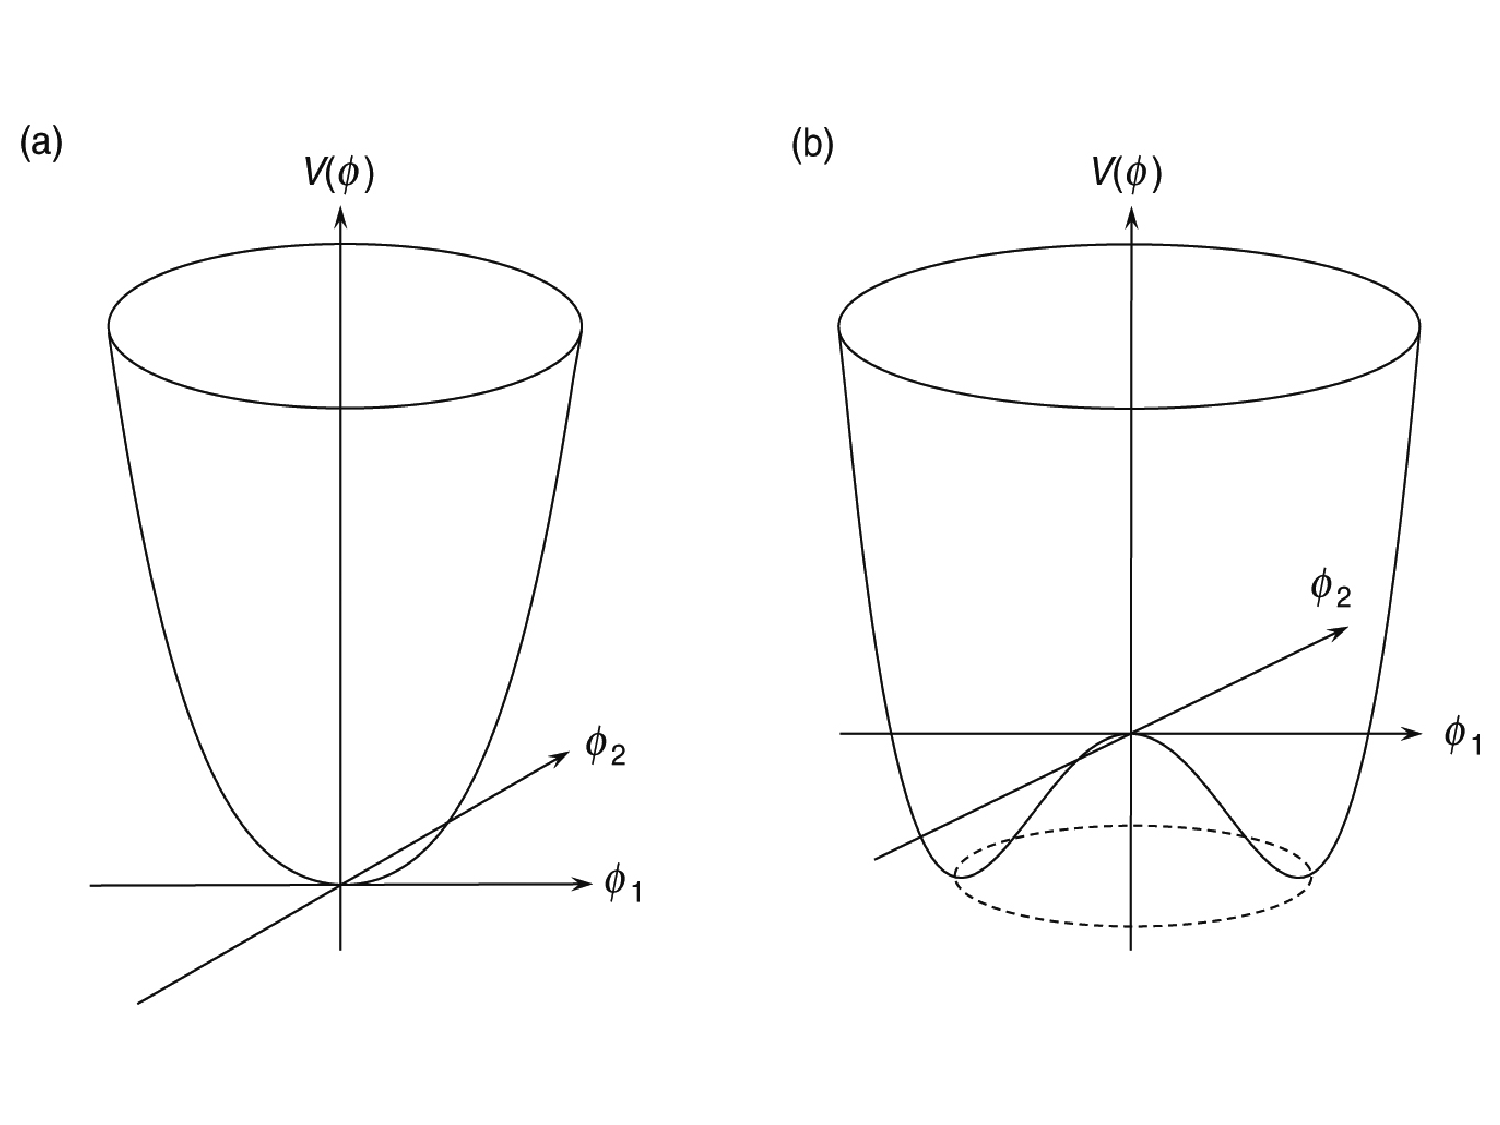
\includegraphics[width=0.8\linewidth]{figs/symm_break.pdf}
\caption{Linear sigma model potential for $N=2$. In (a) the $\phi$ field
         mass term $m^2>0$, while (b) gives this potential when
         $m^2$ is replaced by a negative parameter $-\mu^2$.
         Oscillations along the circle of minima in (b) correspond to 
         the $\pi$ field. Oscillations in the radial direction correspond
         to the $\sigma$ field. Image taken from 
         Thompson~\cite{thomson_modern_2013}.}
\label{fig:ssb}
\end{figure}

Let's try to gain some geometric intuition for this phenomenon. 
Looking at eq.~\eqref{eq:phidir}, we see that in $\phi$ space, the $\sigma$
field corresponds to oscillations of $\phi$ orthogonal to the $N-1$
dimensional hypersurface, while the massless $\pi_k$ fields
corresponds to oscillations along the hypersurface. 
An example with $N=2$ is shown in Figure~\Ref{fig:ssb}. 
If we take the ground state vector~\eqref{eq:phidir} and hit it with
$\text{O}(N)$, it will be rotated somewhere else on the hypersurface.
The subgroup $\text{O}(N-1)$ hits the first $N-1$ components of the
ground state, which are all 0, thereby leaving it unchanged.
In the original $\phi^4$ theory with
$m^2>0$, the ground state vector was 0, so the $\text{O}(N)$ symmetry
was also a symmetry of the ground state. After SSB, $\text{O}(N)$ changes 
the ground state vector in general,
which is why we say the symmetry is broken. Generally any symmetry
respected by the Lagrangian but not by the ground state vector
is a broken symmetry.

In the linear sigma model, massless $\pi$ particles appeared after
SSB. This is a special example of a general result
known as Goldstone's theorem. The generated massless particles are
referred to as \index{Goldstone!boson}{\it Goldstone bosons}. 
Many light bosons can be interpreted
as approximate Goldstone bosons; as we will see in Section~\Ref{sec:cscont},
the pion can be viewed in this manner.
\begin{theorem}{Goldstone's theorem}{}
\index{Goldstone!theorem}
Consider a Lagrangian of the form
$$
  \Lagr=(\text{kinetic term for $\phi$})+
        (\text{terms independent of $\phi$})-V(\phi),
$$
where $\phi$ is the $N$-dimensional vector of real, scalar fields
$\phi_k$, and $\Lagr$ is invariant under a continuous, global
transformation of $\phi$ with generators $T^a$. Then for every
spontaneously broken generator there exists a corresponding
Goldstone boson. 
\begin{proof}
  Let $\phi_\text{min}$ be a constant field minimizing $V$. Expanding
  $V$ about this minimum we get to leading order
  $$
    V(\phi)= V(\phi_\text{min})
     +\frac{1}{2}
      (\phi-\phi_\text{min})_i(\phi-\phi_\text{min})_j\,
      \frac{\partial^2 V}{\partial\phi_i\partial\phi_j}
       \Big|_{\phi=\phi_\text{min}}.
  $$
  The differences $\phi-\phi_\text{min}$ give the new fields of the
  theory after SSB; for example in the linear sigma model this difference
  is, from equations~\eqref{eq:phidir} and \eqref{eq:phishift},
  $$
    \phi-\phi_\text{min}=(\pi_1,...,\pi_{N-1},\sigma).
  $$
  Therefore the coefficient of the quadratic term is a symmetric matrix
  whose eigenvalues give the masses of these fields. If we can prove
  that each broken generator implies a zero eigenvalue for this matrix,
  we are done.
  The kinetic term for $\phi$ is already invariant under the global
  transformation, so if $\Lagr$ is invariant, it follows that $V$ must
  be as well. Then we can write
  $$
    V\left((\id-i\omega^aT^a)\phi\right)=V(\phi),
  $$
  where $\omega$ is some infinitesimal parameter. Expanding to linear
  order yields
  $$
    \frac{\partial V}{\partial\phi_j}(T^a\phi)_j=0.
  $$
  Differentiating the above with respect to $\phi_i$ and evaluating at
  $\phi_\text{min}$ gives
  $$
     \frac{\partial^2 V}{\partial\phi_i\partial\phi_j}
      \Big|_{\phi=\phi_\text{min}}(T^a\phi_\text{min})_j=0,
  $$
  i.e. $T^a\phi_\text{min}$ is annihilated by the mass matrix. 
  If $T^a$ is a broken generator, we have $T^a\phi_\text{min}\neq0$,
  so the above equation implies $T^a\phi_\text{min}$ is an
  eigenvector of the mass matrix with eigenvalue zero.
\end{proof}
\end{theorem}

%In the basis that diagonalizes the mass matrix, the eigenvectors correspond
%to different fields, each with a mass equal to its corresponding eigenvalue.
%
%If you hit the VEV with a broken symmetry, it will rotate it. In the
%$N=2$ linear sigma model, the broken O(2) symmetry rotates the VEV.
%
%Even if it's not clear how the pions in the first case rise from this
%procedure, the important thing is that it guarantees some field
%eigenvectors of M^2, which have 0 eigenvalue. 

\section{Chiral symmetry in the continuum}\label{sec:cscont}
\index{chiral symmetry}

In the continuum, the massless fermion action for a single flavor reads
\begin{equation}
S_F=\int\dd[4]{x}\Lagr_F=\int\dd[4]{x}\bar{\psi}\slashed{D}\psi. 
\end{equation}
We refer to $\slashed{D}$ as the {\it massless Dirac operator}. A 
{\it chiral rotation} of the fermion fields is a transformation
mapping
\begin{equation}
  \psi\to e^{i\alpha\gamma_5}\psi~~~~\text{and}~~~~
  \bar{\psi}\to\bar\psi e^{i\alpha\gamma_5},
\end{equation}
where $\alpha\in\mathbb{R}$. This is probably called a chiral rotation
because $\gamma_5$ is used to define the operators~\eqref{eq:projdef},
which project out the left-handed and right-handed components of the
fermion field according to eq.~\eqref{eq:projact}. Using identity 2 of
Proposition~\Ref{prp:gammatech}, we find that $\Lagr_F$ transforms under this
rotation as
\begin{equation}
  \Lagr_F\to\bar{\psi}e^{i\alpha\gamma_5}\slashed{D}e^{i\alpha\gamma_5}\psi
         =\bar{\psi}e^{i\alpha\gamma_5}e^{-i\alpha\gamma_5}\slashed{D}\psi
         =\Lagr_F,
\end{equation}
i.e. it is invariant under chiral rotations. Using
Proposition~\Ref{prp:projection}, one can decompose $\Lagr_F$ into its
left-handed and right-handed parts as
\begin{equation}
  \Lagr_F=\bar{\psi}_L\slashed{D}\psi_L
         +\bar{\psi}_R\slashed{D}\psi_R,
\end{equation}
and we colloquially say that the chiral components of
$\Lagr_F$ ``do not talk to each other."
If one were to include a mass term in $\Lagr_F$, it would decompose as
\begin{equation}
  m\bar{\psi}\psi=m\left(\bar{\psi}_R\psi_L+\bar{\psi}_L\psi_R\right),
\end{equation}
which mixes the chiral components, thereby breaking chiral symmetry.
This is why one refers to the limit $m\to0$ as the {\it chiral limit}.

We now generalize these ideas to $N_f$ flavors of fermion. In Gattringer
and Lang eq.~(7.11), they write the fermion action as
\begin{equation}\label{eq:nfact}
  S_F=\int\dd[4]{x}\Lagr_F=\int\dd[4]{x}
         \bar{\psi}\left(\slashed{D}+M\right)\psi,
\end{equation}
where $M$ is the {\it mass matrix}\index{mass matrix}
\begin{equation}
  M~``="~\diag(m_1,m_2,...,m_{N_f})
\end{equation}
acting in flavor space. $M$ cannot be a $N_f\times N_f$ matrix, because
we have defined $\gamma^\mu$ as a $4\times4$ matrix. The only way adding 
these matrices makes sense is if $M$ is a $4N_f\times4N_f$ matrix, i.e. if
\begin{equation}
  M=\left(\begin{array}{cccc}
      m_1\id_4 &          &        & \\
               & m_2\id_4 &        & \\
               &          & \ddots & \\
               &          &        & m_{N_f}\id_4
    \end{array}\right).
\end{equation}
Then $\psi$ must be a $4N_f$ vector (in the mathematical sense, not 
in the Lorentz transformation sense) looking something like
\begin{equation}
  \psi=\colvec{4}{\psi_1}{\psi_2}{\vdots}{\psi_{N_f}},
\end{equation}
where each $\psi_i$ is a 4-component Dirac spinor, and presumably when
we write $\gamma^\mu$ in eq.~\eqref{eq:nfact} what we really mean is
\begin{equation}
  \gamma^\mu=\gamma^\mu\id_{N_f}
            =\left(\begin{array}{cccc}
               \gamma^\mu &            &        & \\
                          & \gamma^\mu &        & \\
                          &            & \ddots & \\
                          &            &        & \gamma^\mu
               \end{array}\right).
\end{equation}
I pray the reader forgives the notational perversion in the above equation.

In the chiral limit, the action eq.~\eqref{eq:nfact} is again invariant under
chiral rotations, also in this context called {\it axial vector rotations},
taking the form
\begin{gather}
  \label{eq:SUNfc}
  \psi\to e^{i\alpha\gamma_5 T^a}\psi,\qquad
    \bar{\psi}\to\bar{\psi}e^{i\alpha\gamma_5 T^a}, \\
  \label{eq:U1A}
  \psi\to e^{i\alpha\gamma_5 \id}\psi,\qquad
    \bar{\psi}\to\bar{\psi}e^{i\alpha\gamma_5 \id},
\end{gather}
where the $T^a$ are the $N_f^2-1$ generators of $\SU(N_f)$,
$\id\equiv\id_{4N_f}$, and again $\alpha\in\mathbb{R}$.
In this limit the action is also invariant under the
{\it vector transformations}
\begin{gather}
  \label{eq:SUNf}
  \psi\to e^{i\alpha T^a}\psi,\qquad
    \bar{\psi}\to\bar{\psi}e^{-i\alpha T^a}, \\
  \label{eq:U1V}
  \psi\to e^{i\alpha \id}\psi,\qquad
    \bar{\psi}\to\bar{\psi}e^{-i\alpha \id}.
\end{gather}
This invariance under the above two equations extends to the case of degenerate
masses, when $m_1=m_2=...=m_{N_f}\equiv m$, and is the familiar isospin
symmetry generalized to $N_f$ flavors. The symmetry~\eqref{eq:U1V} holds for
arbitrary masses, and the conserved quantity is the {\it baryon number}
\begin{equation}
    B=\frac{1}{3}(n_q-n_{\bar{q}}).
\end{equation}
You can see why it's called baryon number: A baryon is made of 3
quarks, and hence has $B=1$. Anti-quarks have $B=-1$, and
mesons have $B=0$.

Returning once again to the massless limit, the invariance of the action under
eqs.~\eqref{eq:SUNfc}, \eqref{eq:U1A}, \eqref{eq:SUNf}, and \eqref{eq:U1V}
represents the global symmetry group
\begin{equation}\label{eq:SMfglobal}
  \SU(N_f)_L\times\SU(N_f)_R\times\U(1)_V\times\U(1)_A.
\end{equation}
Breaking the global symmetry group~\eqref{eq:SMfglobal} has important
implications in QCD phenomonology. For example we will show that in the
quantized, massless theory the fermion determinant changes
under~\eqref{eq:U1A}, breaking the $\U(1)_A$ symmetry explicitly. The remaining
symmetry is
\begin{equation}\label{eq:SMglobalbUA}
  \SU(N_f)_L\times\SU(N_f)_R\times\U(1)_V.
\end{equation}
If the fermion masses are degenerate, the symmetry $\SU(N_f)_L\times\SU(N_f)_R$
breaks to its subgroup $\SU(N_f)_V$. Now the remaining symmetry is
\begin{equation}
  \SU(N_f)_V\times\U(1)_V.
\end{equation}
Finally allowing non-degenerate masses breaks the symmetry further. 
There remains
\begin{equation}
  \underbrace{\U(1)_V\times\U(1)_V\times...\times\U(1)_V}_\text{$N_f$ times}.
\end{equation}

The typical QCD scale is $\sim1~\text{GeV}$ (think protons, which have a 
mass of about 940~MeV) so the $u$, $d$, and $s$ quarks have masses that
are relatively small (about 5~MeV, 5~MeV, and 100~MeV, respectively).
Since these masses are so close to zero on this scale, we can say that
when $N_f=2$, and partly for $N_f=3$, eq.~\eqref{eq:SMglobalbUA} is
an approximate symmetry. If the $u$ and $d$ quarks were massless, this symmetry
would be exact, and it can be argued~\cite{gattringer_quantum_2010} that
a nucleon and its negative parity partner should have the same mass. 
However one finds the negative parity nucleon to have
a mass of about 1535~MeV, and this difference of about 600~MeV is too large to
be explained by the slight breaking due to the $u$ and $d$ masses. We
conclude that something else is happening. This something is called 
{\it spontaneous chiral symmetry breaking}, and it comes out of the
dynamics of QCD. If quarks were massless, the pions would arise as 
the Goldstone bosons of chiral SSB; hence we refer to pions as 
``would-be" Goldstone bosons.

% Berg insight relating this stuff to pure SU(N): in our simulations we sample
% A_\mu, so \partial_\mu + iA_\mu is well defined, which means
% \gamma_\mu(\partial_\mu +iA_\mu) is well defined, which is the Dirac
% operator. The Dirac operator is a matrix, so as long as it's diagonalizable
% you can find eigenvectors. The fact that our action is pure SU(N) only really
% changes the distribution of the A_\mu.
%\section{Chiral symmetry on the lattice}\label{sec:cslat}
%For light quarks, the fermion action is roughly invariant under the global
%symmetry~\eqref{eq:SMglobalbUA}. Experimental findings do not reflect this
%chiral symmetry, so we conclude it is broken spontaneously by QCD dynamics.
%The small pion masses can be attributed to a further, slight breaking
%of this symmetry. Since chiral symmetry breaking is important in high
%energy phenomenology, it is worth implementing on the lattice.

\section{Neutrino Oscillations}
This section summarizes the experiments and observations that led to the belief
that neutrinos have mass. First the solar neutrino problem and early solar
neutrino experiments are discussed. The atmospheric neutrino problem is
discussed. Next the theory behind neutrino oscillations is explained, along
with a possible Standard Model (SM) mechanism giving neutrinos mass. Recent
experiments supporting the neutrino oscillation hypothesis are discussed,
along with future possibilities for neutrino physics research.

\subsection{The Solar Neutrino Problem}

\begin{figure}
  \centering
  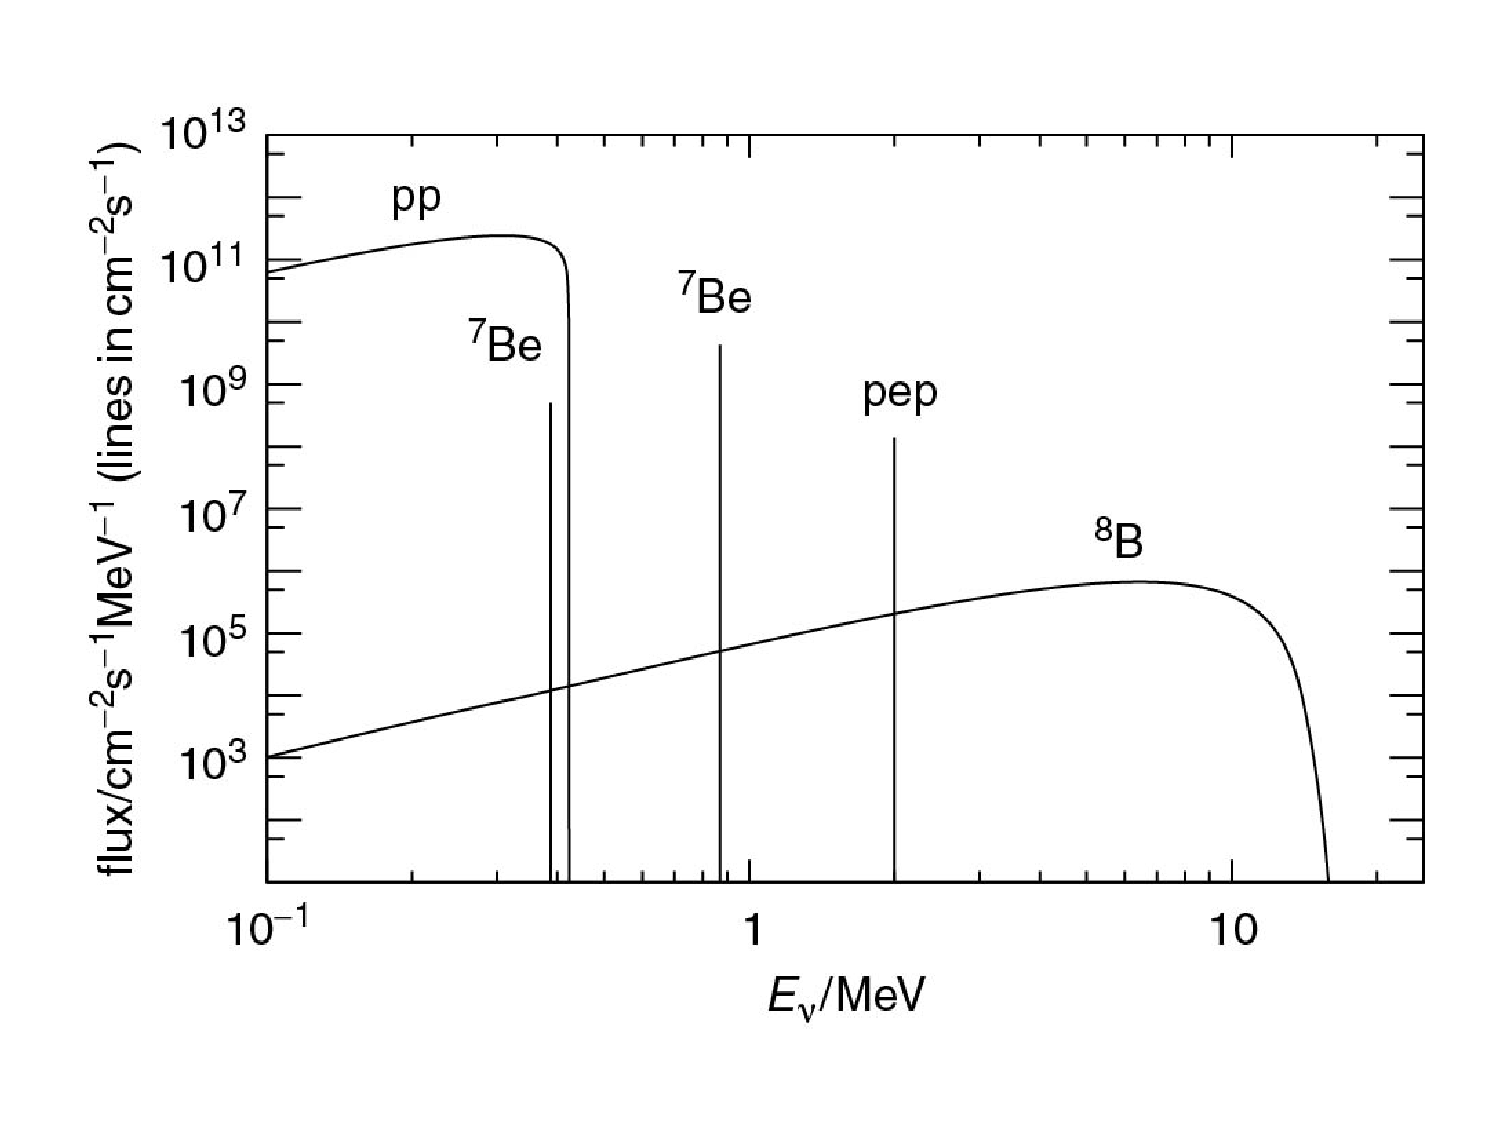
\includegraphics[height=0.33\textheight,keepaspectratio]
                {pictures/t13_3.pdf}
  \caption{Solar neutrino flux and energy of several processes in the sun.
           Image taken from Thomson Figure 13.3 \cite{thomson_modern_2013}.}
\end{figure}
Roughly $2\times10^{38}$ $\nu_e$ are produced by nuclear fusion in the sun
each second. One of the main processes by which this occurs is the pp-cycle,
$\text{p}+\text{p}\to\text{D}+\text{e}^++\nu_e$. However experiments detecting
solar neutrinos tend to focus on rarer reactions, such as the
$\prescript{7}{}{\text{Be}}$ electron capture process, pep-process, and
$\prescript{8}{}{\text{B}}$ $\beta$-decay, which are, respectively,
\begin{equation}
  \begin{aligned}
    \prescript{7}{}{\text{Be}}+\text{e}^-&\to\prescript{7}{}{\text{Li}}+\nu_e,
    \\
    \text{p}+\text{e}^-+\text{p}&\to\prescript{2}{}{\text{H}}+\nu_e, 
    \\
    \prescript{8}{5}{\text{B}}&\to\prescript{8}{4}{\text{Be}}^*+\text{e}^+
      +\nu_e.
  \end{aligned}
\end{equation}
As illustrated in Figure 1, these processes tend to produce neutrinos of higher
energies than the pp-cycle, which allows the neutrinos to overcome kinematic
barriers that would otherwise preclude them from participating in the
interactions used to detect them.
The Standard Solar Model (SSM) allows us to predict how many electron neutrinos
we expect to see. However the results of the first experiments measuring solar
neutrino flux were somewhat unexpected.

\subsubsection{Radiochemical experiments}
Ray Davis, Jr. and his collaborators started the first experiment to detect
solar neutrinos. The Homestake experiment, based in a mine in South Dakota,
had a 615 ton tank full of dry-cleaning fluid, $\text{C}_2\text{Cl}_4$,
which was chosen for the interaction mentioned below.
Mines are prime real estate for neutrino experiments because being underground
helps isolate them from cosmic rays. The number of captured solar neutrinos
was measured by counting the $\prescript{37}{}{\text{Ar}}$ atoms produced in
the process
\begin{equation}
  \nu_e+\prescript{37}{17}{\text{Cl}}\to
        \prescript{37}{18}{\text{Ar}}+\text{e}^-.
\end{equation}
The minimum energy an electron neutrino needs to participate in the above
process is about 0.81 MeV, which excludes neutrinos produced by the pp-cycle.
Although a huge number of electron neutrinos exit the sun, the SSM
predicted a modest 1.7 interactions per day. The findings
of Homestake were presented in 1968: Merely $0.48\pm0.04$ daily interactions
were found!

Later radiochemical experiments used gallium as a target, and were therefore
sensitive to neutrinos produced in the pp-cycle. The Soviet-American
Gallium Experiment (SAGE) started running in 1989, and appears to still be
collecting data as of March 2015 \cite{G1}. The Gallium Experiment (GALLEX),
which was later succeeded by the Gallium Neutrino Observatory (GNO),
collected data between 1991 and 1997, and was an international project
managed by American, French, German, Italian, Israeli, and Polish scientists.
Both of these experiments confirmed the deficit of solar neutrinos; this
mysterious absence of solar neutrinos became known as the {\it solar
neutrino problem}.

\subsubsection{Water \v{C}erenkov Experiments}
\v{C}erenkov radiation occurs whenever a charged particle passes through a
dielectric medium at a speed greater than the phase speed of light in that
medium. The particle polarizes the medium, then travels away from that
disturbance faster than the electromagnetic field can react, leaving
a wake where those disturbances constructively interfere. Elementary
geometry shows that if the medium has index of refraction $n$, the angle
at which this radiation is emitted is given by $\co=1/n\beta$. Water
\v{C}erenkov detectors work by measuring this angle as leptons propagate
through water. This in turn gives a measure of $\beta$, and hence the energy.

\begin{figure}
  \centering
  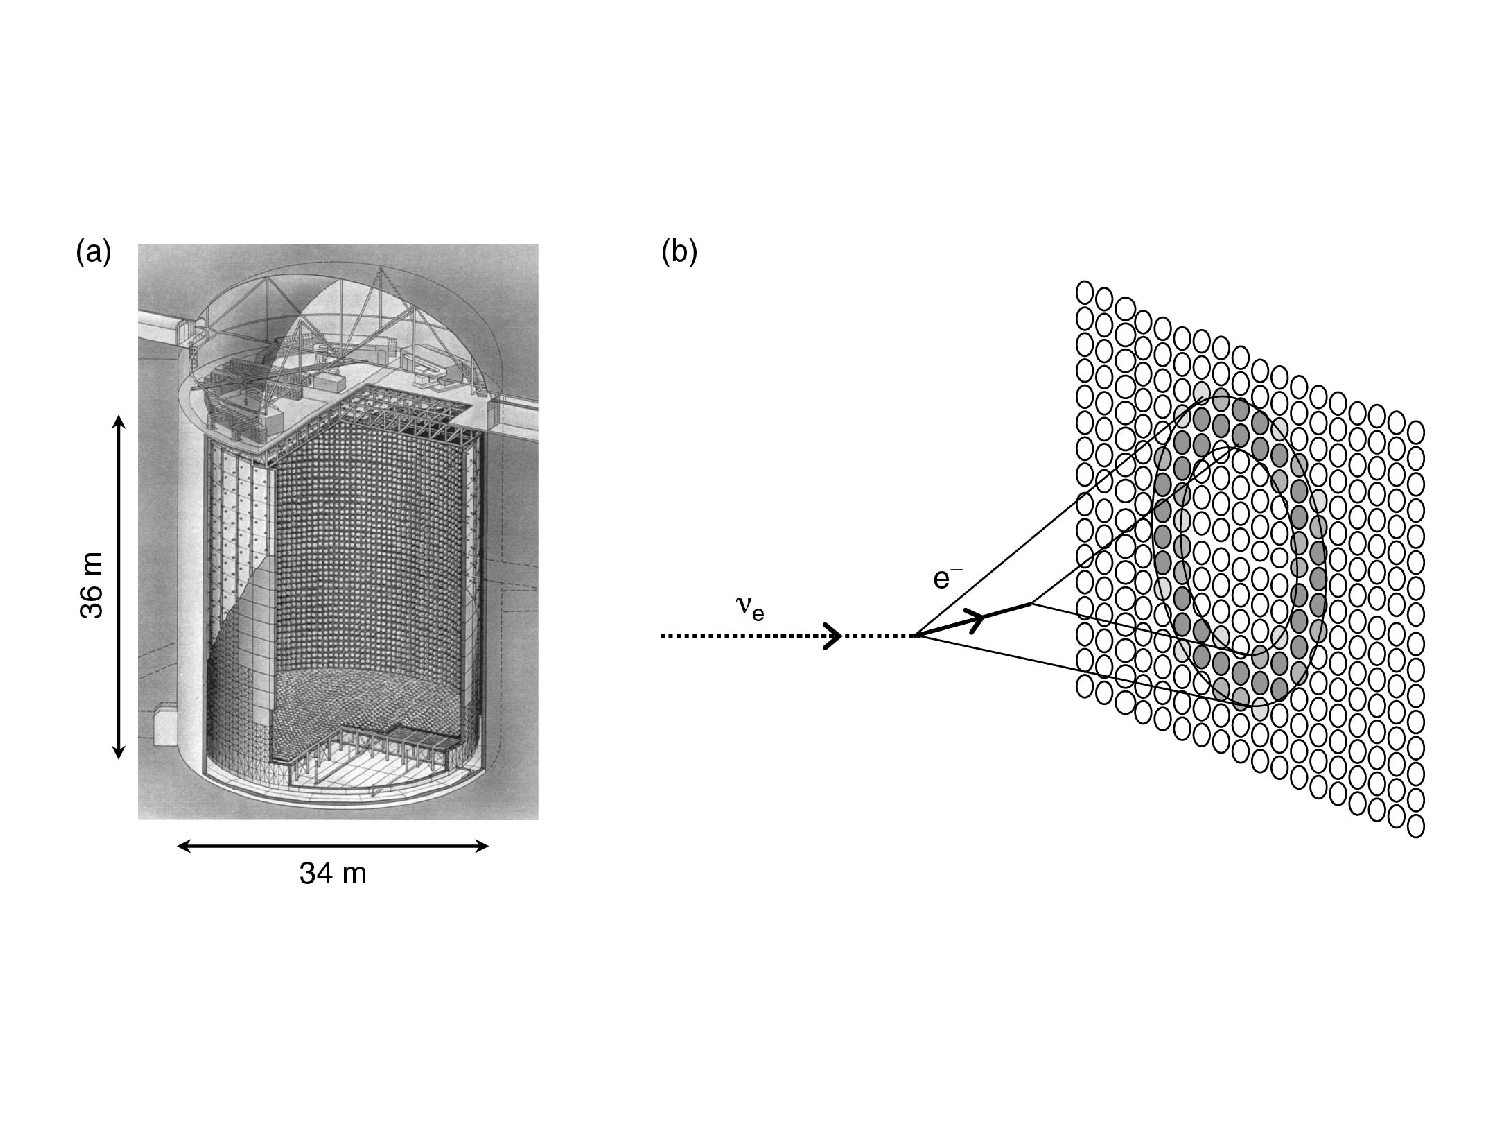
\includegraphics[width=0.85\textwidth,height=0.85\textheight,keepaspectratio]
                {pictures/t13_4.pdf}
  \vspace*{-10mm}
  \caption{(a) Schematic of the Super-K tank. (b) An example of an electron
           projecting a \v{C}erenkov ring on PMTs. Image taken
           from Thomson Figure 13.4 \cite{thomson_modern_2013}.}
\end{figure}

The Kamioka Nucleon Decay Experiment (KamiokaNDE or usually Kamiokande) was
originally a project to study proton decay. In 1988 it was
upgraded, giving it the ability to study solar neutrinos. It was upgraded
again in 1996, donning the name Super Kamiokande (Super-K), with the intent
of obtaining higher statistics than Kamiokande. Super-K is still running today.
Located 1 km underground in the Kamioka area of Gifa Prefecture, Japan,
the Super-K detector consists of a 50 kiloton water tank viewed by 11,146
photo multiplier tubes (PMTs). As charged leptons pass through the water,
they project rings of \v{C}erenkov light on the walls of the detector. The
center-of-mass (CM)
frame is boosted in the direction of the neutrino, which means that the
electron direction is very close to the neutrino direction. This setup
allows experimentalists to not only detect neutrino energies down to
approximately 5 MeV, but also detect particle orientations, which gives Super-K
an advantage over radiochemical experiments.
The neutrinos are detected through the elastic scattering (ES) process
$\nu_ee^-\to\nu_ee^-$. One might expect to also see neutrinos interact
using oxygen, in particular through the charged current (CC) process
$\nu_e+\prescript{16}{8}{\text{O}}\to\prescript{16}{9}{\text{F}}+e^-$.
But oxygen is more stable than the fluorine isotope, making the process
kinematically forbidden to the relatively low energy solar neutrinos. The 5
MeV threshold, which is a result of radioisotope $\beta$ decay background,
 makes Super-K primarily sensitive to neutrinos produced by
the $\prescript{8}{}{\text{B}}$ process.

The left plot of Figure 3 is a graph of the electron direction with
respect to the
direction of the sun. The largest number of events occurred near $\co=1$,
which provides strong evidence that a large flux of neutrinos comes from the
sun. Just as its predecessors, Super-K experienced an electron neutrino
deficit, finding only $0.474\pm0.03$ of the number of electron neutrinos
predicted by the SSM.

Homestake, Super-K, and other neutrino experiments clearly demonstrated
a dearth of solar electron neutrinos. The Sudbury Neutrino Observatory (SNO)
in Canada took these experiments a step further by measuring the
electron neutrino flux and total neutrino flux from the sun. SNO had a 12m
diameter tank filled with 1 kiloton of $\text{D}_2\text{O}$, which was used
because deuteron has a small binding energy compared to the energies of
neutrinos produced by $\prescript{8}{}{\text{B}}$. Electron neutrinos can then
be detected through
$\nu_e+\text{D}\to\text{e}^-+\text{p}+\text{p}$,
the CC interaction, and neutrinos of all flavors
interact with the deuteron via the neutral current (NC) interaction
$\nu_\ell+\text{D}\to\nu_\ell+\text{n}+\text{p}$ and ES interactions. The NC
interaction is equally sensitive to all flavors of neutrino, but the ES
interaction is more sensitive to electron neutrinos because $\nu_\mu$ and
$\nu_\tau$ only interact through the NC ES process. In total the interaction
rates obey
\begin{equation}
  \begin{aligned}
    \text{CC rate}&\propto\Phi(\nu_e), \\
    \text{NC rate}&\propto\Phi(\nu_e)+\Phi(\nu_\mu)+\Phi(\nu_\tau), \\
    \text{ES rate}&\propto\Phi(\nu_e)+0.154\big(\Phi(\nu_e)+\Phi(\nu_e)\big).
  \end{aligned}
\end{equation}

For the CC interaction, the
emitted electron is detected through its \v{C}erenkov ring. In the CM frame
the direction of the neutrino relative to the electron is nearly isotropic, and
because the neutrino energy is much smaller than the deuteron mass, the
electron orientation is essentially uncorrelated with the sun's direction.
The ES interaction is also detected through \v{C}erenkov rings, but these
leptons correlate with the sun's direction as in the Super-K. For the NC
interaction, the produced neutron is eventually captured in the process
$\text{n}+\prescript{2}{1}{\text{H}}\to\prescript{3}{1}{\text{H}}+\gamma$.
The photon then produces electrons through subsequent interactions that are
then detected by \v{C}erenkov rings. Ultimately SNO found
\begin{equation}
  \begin{aligned}
    \Phi(\nu_e)&=(1.76\pm0.10)\times10^{-6}~\text{cm}^{-2}\text{s}^{-2} \\
    \Phi(\nu_\mu)+\Phi(\nu_\tau)
               &=(3.41\pm0.63)\times10^{-6}~\text{cm}^{-2}\text{s}^{-2},
  \end{aligned}
\end{equation}
The theoretical prediction of the electron neutrino flux was
\begin{equation}
  \Phi(\nu_e)_{theory}=(5.1\pm0.9)\times10^{-6}~\text{cm}^{-2}\text{s}^{-1}, 
\end{equation}
so we see that $\Phi(\nu_e)_{theory}=\Phi(\nu_e)+\Phi(\nu_\mu)+\Phi(\nu_\tau)$
within error. Thus SNO showed that the total
neutrino flux was consistent with the theoretical expectation as long as
one allows the neutrino flux from the sun to include muon and tau neutrinos.
But these flavors of neutrinos aren't produced in the sun; therefore SNO also
provided real evidence of neutrino oscillations.
A plot showing the confidence bands of the different processes for data
generated by SNO is shown on the right of Figure 3.

\begin{figure}
  \centering
  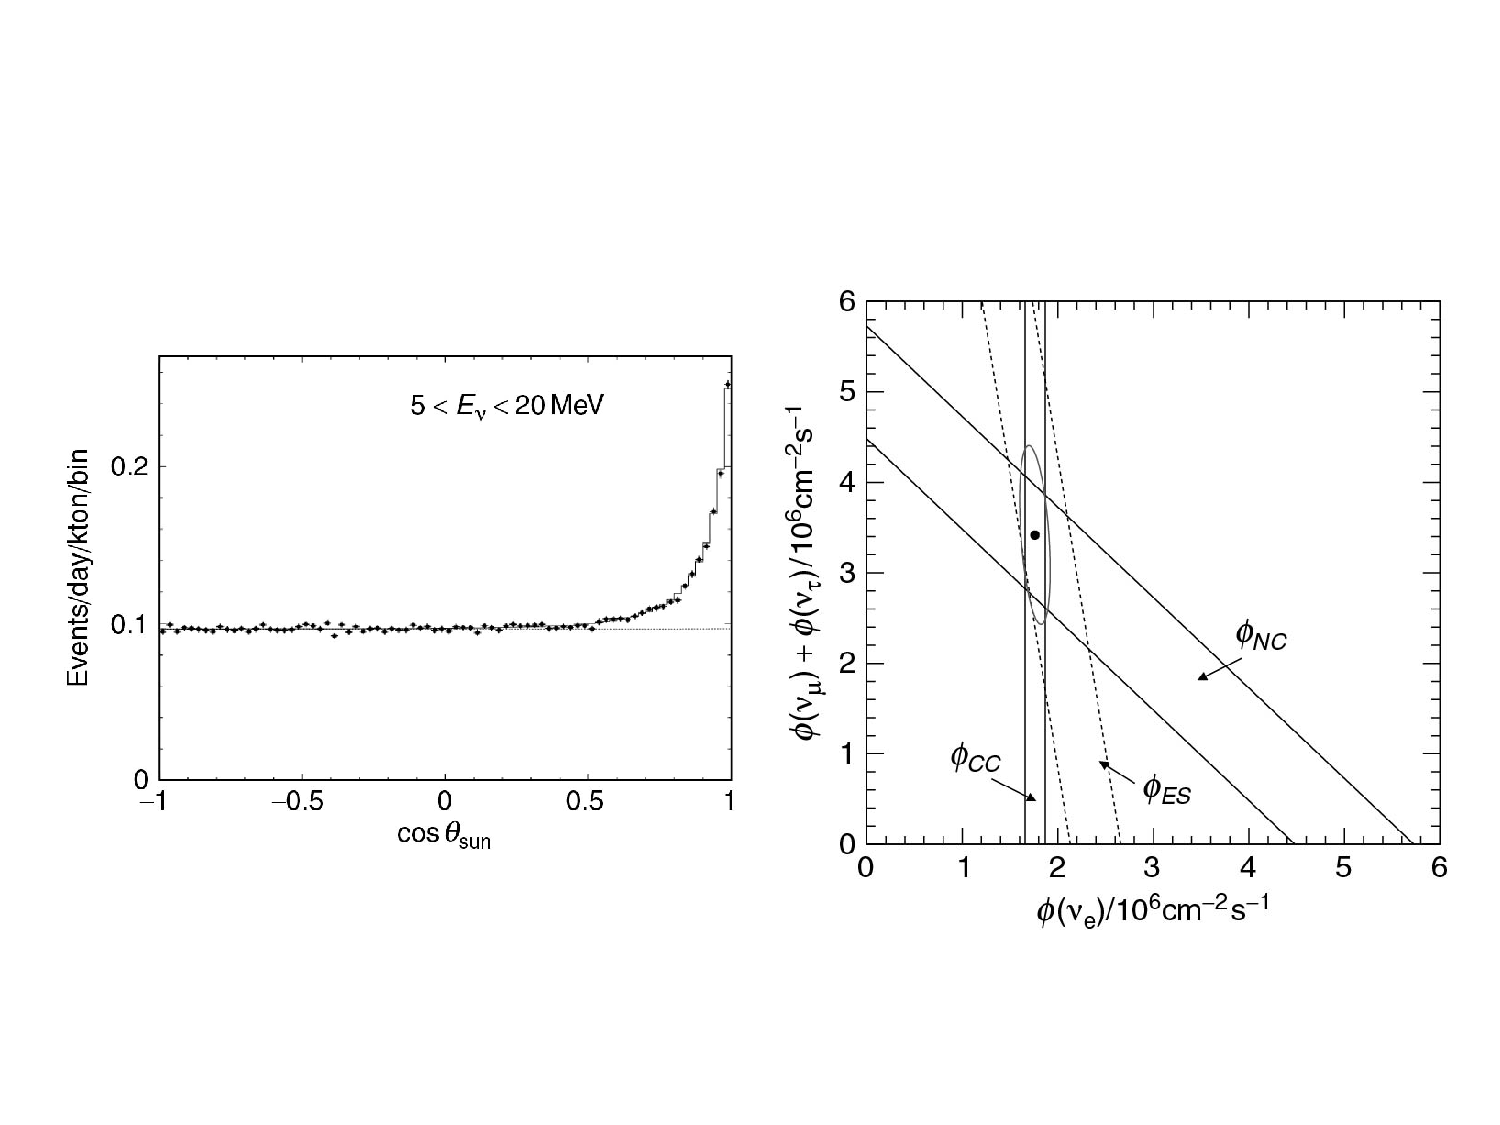
\includegraphics[width=0.85\textwidth,height=0.85\textheight,keepaspectratio]
                {pictures/t13_6&8.pdf}
  \vspace*{-10mm}
  \caption{Left: Super-K neutrino data plotted against the cosine of the
           angle of the electron with respect to the sun. Right: Constraints
           on neutrino fluxes from SNO data. The bands indicate one standard
           deviation, and the 68\% confidence ellipse is shown. Images taken
           from Thomson Figures 13.6 and 13.8 \cite{thomson_modern_2013}.}
\end{figure}

These early discoveries about neutrinos weren't merely surprising; they
created a new and burgeoning area of study in high energy physics
that lends important
insight to the nature of SM neutrinos. Discoveries about neutrinos tend
to generate a lot of excitement.
In fact in 2002, Ray Davis and Masatoshi Koshiba each received 1/4 of
the Nobel Prize for their involvement in neutrino detection, the former
due to Homestake and the latter due to Super-K. Earlier this year,
Takaaki Kajita and Arthur B. McDonald split the Nobel Prize for their
stakes in the Super-K and SNO experiments, respectively.

\subsection{The Atmospheric Neutrino Problem}
Cosmic rays, which consist mostly of protons and alpha particles, interact with
particles in the earth's atmosphere. Secondary particles emitted in these
interactions will sometimes decay and produce an {\it atmospheric} neutrino,
provided their energy is low enough ($\lesssim$2 GeV). The atmospheric neutrinos
are then produced via
\begin{equation}
  \begin{aligned}
    \text{p}+N&\to\pi^\pm+X, \\
    \pi^\pm&\to\mu^\pm+\nu_\mu(\bar{\nu}_\mu), \\
    \mu^\pm&\to e^\pm+\nu_e(\bar{\nu}_e)+\bar{\nu}_e(\nu_\mu).
  \end{aligned}
\end{equation}
Assuming the neutrino flavor doesn't change on its journey to the detector,
the above sequence of processes implies
\begin{equation}
  \mathcal{R}\equiv\frac{N_{\nu\mu}+N_{\bar{\nu}\mu}}
                           {N_{\nu e}+N_{\bar{\nu}e}}\approx2,
\end{equation}
where $N_i$ indicates the number of particles of type $i$.
It is difficult to determine an exact value for $\mathcal{R}$ because it is
affected by many factors, including solar activity and geomagnetic cut-off.
Therefore to create a quantity independent of external effects, we define
\begin{equation}
  \mathcal{R}'\equiv\frac{\mathcal{R}}{\mathcal{R}_\text{MC}},
\end{equation}
where $\mathcal{R}_\text{MC}$ is obtained using Monte Carlo simulations instead
of observed data. A drawback to $\mathcal{R}'$ is that it cannot distinguish
between an abundance of electrons and a deficit of muons.
In 1986, the first experiment to discover a discrepancy between the number of
observed and expected atmospheric neutrinos was the Irvine-Michigan-Brookhaven
detector
(IMB), which was located in a salt mine owned by Morton on the shore of Lake
Erie, Ohio.  Shortly thereafter in 1988, Kamiokande confirmed this deficit.
The next two experiments to investigate this phenomenon, Fr\'ejus and NUSEX,
actually were unable to reproduce this finding. As a result many physicists
believed the discrepancy was due to systematic errors originating in our poor
understanding of neutrino interactions with iron and water. The issue was
resolved when the Soudan2 experiment reaffirmed the findings of IMB and
Kamiokande. But the most convincing results came from Super-K, which showed
that the deficit of neutrinos depends on the zenith angle.

\begin{figure}
  \centering
  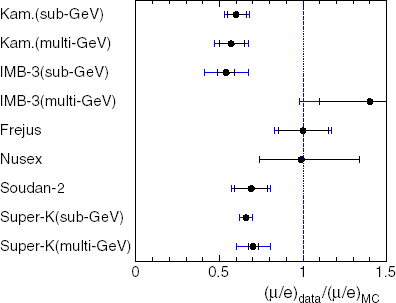
\includegraphics[width=0.85\textwidth,height=0.25\textheight,keepaspectratio]
                {pictures/dblratio.jpg}
  \vspace*{10mm}
  \caption{Plot summarizing the values of $\mathcal{R}'$ as found by early
           neutrino experiments. Image taken from Figure 11 on T2K experiment
           webpage \cite{T2}.}
\end{figure}

\subsection{Theory of Neutrino Oscillations}
Thankfully, both the atmospheric and solar neutrino problems are resolved
neatly by neutrino oscillations.
Here we briefly explain the theory behind neutrino oscillations as well as a
model for how neutrinos gain mass. In the following, we use $x$ to denote
the four-vector of a particle's space-time position.

The {\it mass eigenstates} $\nu_1$, $\nu_2$, and $\nu_3$ of the free particle
Hamiltonian are its physical states of definite mass; i.e., they are the
eigenstates of the Hamiltonian. Meanwhile the {\it weak eigenstates} $\nu_e$,
$\nu_\mu$, and $\nu_\tau$ are the eigenstates corresponding to particles
produced in weak interactions. There is no a priori reason to assume that these
are the same set of eigenstates--in general each set forms a basis spanning
the space of physical states. Hence we can relate the bases to each other
through a unitary transformation, represented below as the
Pontecorvo-Maki-Nakagawa-Sakata (PMNS) matrix. We write
\begin{equation}
  \colvec{3}{\nu_e}{\nu_\mu}{\nu_\tau}=
  \left(\begin{array}{ccc}
    U_{e1} & U_{e2} & U_{e3} \\
    U_{\mu 1} & U_{\mu 2} & U_{\mu 3} \\
    U_{\tau 1} & U_{\tau 2} & U_{\tau 3}
  \end{array}\right)
  \colvec{3}{\nu_1}{\nu_2}{\nu_3}
\end{equation}
from which we see that the electron neutrino state, for example, is
a superposition of the mass eigenstates
\begin{equation}
  \label{eq:mix1}
  \ket{\nu_e}=U_{e1}^*\ket{\nu_1}+U_{e2}^*\ket{\nu_2}+U_{e3}^*\ket{\nu_3}.
\end{equation}
Once the neutrino weakly interacts, the wavefunction collapses to a (possibly
different) weak eigenstate. This is believed to be the mechanism by which
neutrinos change flavor.

\subsubsection{The PMNS Matrix}

In general the elements of the PMNS matrix are complex,
so it can be parameterized by eighteen real numbers. However since
$U^\dagger U=\id$, we obtain nine constraints among the elements, which leaves
nine parameters. Hence the matrix can be written in terms of three
mixing angles $\theta_{12}$, $\theta_{23}$, and $\theta_{13}$, and six phases.
Five of these phases can be absorbed in the definitions of neutrino
and charged lepton spinors without modifying weak interaction currents. To
see this note that using the PMNS matrix, a typical weak interaction term can
be written as
\begin{equation}
  -i\frac{g_W}{\sqrt{8}}(\bar{e},\bar{\mu},\bar{\tau})\gamma^\mu(1-\gamma_5)
  \left(\begin{array}{ccc}
    U_{e1} & U_{e2} & U_{e3} \\
    U_{\mu 1} & U_{\mu 2} & U_{\mu 3} \\
    U_{\tau 1} & U_{\tau 2} & U_{\tau 3}
  \end{array}\right)
  \colvec{3}{\nu_1}{\nu_2}{\nu_3}. \\
\end{equation}
We can rephase the PMNS matrix by pulling out two diagonal matrices
of three phases each, one on the left and one on the right. The left matrix
of phases can then be incorporated into the charged lepton phases while the
right matrix of phases is incorporated into the neutrino phases. The reason
that this eliminates five parameters rather than six is that one of these
phases is redundant; indeed, multiplying the PMNS matrix by an overall phase
$\theta$ has no physical consequence, and the other six phases can be
defined relative to $\theta$.

Ultimately we are left with our three angles and one phase, which we will
call $\delta$. The PMNS is then usually cast as something close to a product
of three rotations about orthogonal axes,
\begin{equation}
  \begin{aligned}
    U_{PMNS}&=
    \left(\begin{array}{ccc}
      1 & 0 & 0 \\
      0 & c_{23} & s_{23} \\
      0 & -s_{23} & c_{23}
    \end{array}\right)
    \left(\begin{array}{ccc}
      c_{13} & 0 & s_{13}e^{-i\delta} \\
      0 & 1 & 0 \\
      -s_{13}e^{i\delta} & 0 & c_{13}
    \end{array}\right)
    \left(\begin{array}{ccc}
      c_{12} & s_{12} & 0 \\
      -s_{12} & c_{12} & 0 \\
      0 & 0 & 1
    \end{array}\right)\\
    &=
    \left(\begin{array}{ccc}
      c_{12}c_{13} & s_{12}c_{13} & s_{13}e^{-i\delta} \\
      -s_{12}c_{23}-c_{12}s_{23}s_{13}e^{i\delta} 
       & c_{12}c_{23}-s_{12}s_{23}s_{13}e^{i\delta} & s_{23}c_{13} \\
      s_{12}s_{23}-c_{12}c_{23}s_{13}e^{i\delta} 
       & -c_{12}s_{23}-s_{12}c_{23}s_{13}e^{i\delta} & c_{23}c_{13}
    \end{array}\right),
  \end{aligned}
\end{equation}
where $c_{ij}\equiv \cos\theta_{ij}$ and
$s_{ij}\equiv \sin\theta_{ij}$. As a final note, the above computations
were carried out under the assumption that neutrinos correspond to Dirac
spinors. If they correspond to Majorana spinors, two more degrees of freedom
appear, and we have to multiply the PMNS matrix on the right by a diagonal
matrix with three phases, $\alpha_1/2$, $\alpha_2/2$, and 0.

\subsubsection{Three Flavors}
Let us explore the mechanism behind neutrino oscillation in more detail.
The mass eigenstates propagate as plane waves
\begin{equation}
  \label{eq:evolve1}
  \ket{\nu_i(t)}=\ket{\nu_i}e^{-ip_ix},
\end{equation}
where $1\leq i\leq3$. Suppose that at $x=0$ an electron neutrino
is produced in a weak process and let $\phi_i=p_i~x$. Then from equations
\eqref{eq:mix1} and \eqref{eq:evolve1}, the wavefunction at an arbitrary
space-time point $x$ is
\begin{equation}
  \begin{aligned}
    \ket{\psi(x)}&=U_{e1}^*\ket{\nu_1}e^{-i\phi_1}
                  +U_{e2}^*\ket{\nu_2}e^{-i\phi_2}
                  +U_{e3}^*\ket{\nu_3}e^{-i\phi_3} \\
                 &=U_{e1}^*(U_{e1}\ket{\nu_e}+U_{\mu 1}\ket{\nu_\mu}
                   +U_{\tau 1}\ket{\nu_\tau})e^{-i\phi_1} \\
                 &~~~~~~
                  +U_{e2}^*(U_{e2}\ket{\nu_e}+U_{\mu 2}\ket{\nu_\mu}
                   +U_{\tau 2}\ket{\nu_\tau})e^{-i\phi_2} \\
                 &~~~~~~
                  +U_{e3}^*(U_{e3}\ket{\nu_e}+U_{\mu 3}\ket{\nu_\mu}
                   +U_{\tau 3}\ket{\nu_\tau})e^{-i\phi_3} \\
                 &=\left(U_{e1}^*U_{e1}e^{-i\phi_1}
                    +U_{e2}^*U_{e2}e^{-i\phi_2}
                    +U_{e3}^*U_{e3}e^{-i\phi_3}\right)\ket{\nu_e} \\
                 &~~~~~~
                   +\left(U_{e1}^*U_{\mu 1}e^{-i\phi_1}
                    +U_{e2}^*U_{\mu 2}e^{-i\phi_2}
                    +U_{e3}^*U_{\mu 3}e^{-i\phi_3}\right)\ket{\nu_\mu} \\
                 &~~~~~~
                   +\left(U_{e1}^*U_{\tau 1}e^{-i\phi_1}
                    +U_{e2}^*U_{\tau 2}e^{-i\phi_2}
                    +U_{e3}^*U_{\tau 3}e^{-i\phi_3}\right)\ket{\nu_\tau}.
  \end{aligned}
\end{equation}
We can extract oscillation probabilities from the above equation by projecting
the state vector on weak eigenstates. For instance the probability of finding
that our initial electron neutrino has oscillated into a muon neutrino at $x$ is
\begin{equation}
  \pr{\nu_e\to\nu_\mu}=\left|U_{e1}^*U_{\mu 1}e^{-i\phi_1}
                    +U_{e2}^*U_{\mu 2}e^{-i\phi_2}
                    +U_{e3}^*U_{\mu 3}e^{-i\phi_3}\right|^2.
\end{equation}
Using the unitarity relations among the PMNS matrix elements, along with the
identity
\begin{equation}
  |z_1+z_2+z_3|^2=|z_1|^2+|z_2|^2+|z_3|^2
                  +2\Re{z_1z_2^*+z_1z_3^*+z_2z_3^*},
\end{equation}
the above oscillation probability simplifies to
\begin{equation}
  \begin{aligned}
    \pr{\nu_e\to\nu_\mu}=&
    2\Re{U_{e1}^*U_{\mu 1}U_{e2}U_{\mu 2}^*\left(e^{i(\phi_2-\phi_1)}-1\right)}
     \\&~+
    2\Re{U_{e1}^*U_{\mu 1}U_{e3}U_{\mu 3}^*\left(e^{i(\phi_3-\phi_1)}-1\right)}
     \\&~+
    2\Re{U_{e2}^*U_{\mu 2}U_{e3}U_{\mu 3}^*\left(e^{i(\phi_3-\phi_2)}-1\right)}
     .
  \end{aligned}
\end{equation}
Similarly the electron neutrino survival probability is
\begin{equation}
  \begin{aligned}
    \pr{\nu_e\to\nu_e}=1&+2|U_{e1}|^2|U_{e2}|^2\Re{e^{i(\phi_2-\phi_1)}-1} \\
                        &+2|U_{e1}|^2|U_{e3}|^2\Re{e^{i(\phi_3-\phi_1)}-1} \\
                        &+2|U_{e2}|^2|U_{e3}|^2\Re{e^{i(\phi_3-\phi_2)}-1}.
  \end{aligned}
\end{equation}
To simplify these equations, define phase differences by
\begin{equation}
  \label{eq:phase}
  \Delta_{ji}\equiv\frac{\phi_j-\phi_i}{2}
                  =\frac{(m_j^2-m_i^2)|\vec{x}|}{4E_\nu}.
\end{equation}
The equality follows from the facts that
\begin{equation}
  \phi_j-\phi_i=(E_j-E_i)t-(|\vec{p}_1|-|\vec{p}_2|)|\vec{x}|
\end{equation}
and $t\approx|\vec{x}|$ since $\beta\approx1$.
Using the phase differences, we can recast the electron survival probability as
\begin{equation}
  \label{eq:esurv}
  \begin{aligned}
    \pr{\nu_e\to\nu_e}=1&-4|U_{e1}|^2|U_{e2}|^2\sin^2\Delta_{21} \\
                        &-4|U_{e1}|^2|U_{e3}|^2\sin^2\Delta_{31} \\
                        &-4|U_{e2}|^2|U_{e3}|^2\sin^2\Delta_{32}.
  \end{aligned}
\end{equation}
We see that when the phase differences are near zero, the survival probability
is close to 1. Since the masses of the neutrinos are small compared to their
energies, the mass differences are also small. This means that the survival
probability is nearly unity, except over large distances, which proffers
an explanation for why these oscillations did not manifest in early neutrino
beam experiments. We also see that if neutrinos are massless and this model is
correct, then there can be no oscillations. Since we have good evidence that
neutrino oscillations occur, and because we also have evidence that this model
accurately describes them, it follows that neutrinos have nonzero,
non-degenerate masses.

\subsubsection{Two Flavors}
The above formalism gives the general treatment of neutrino oscillations
of three flavors, but for the present neutrino data, it is essentially correct
to assume only two flavors \cite{T1}. For this reason, we will briefly review
two flavor oscillations.

When there are two flavors, the relationship between the mass and weak bases
can be parameterized by a mixing angle $\theta$, which is analogous to the
Cabibbo angle. We have
\begin{equation}
  \colvec{2}{\nu_e}{\nu_\mu}=
  \left(\begin{array}{cc}
    \co & \s \\
    -\s & \co
  \end{array}\right)
  \colvec{2}{\nu_1}{\nu_2}.
\end{equation}
Again assuming the particle starts off as an electron neutrino at $x=0$, and
following the same procedure as before, we find the wavefunction at a general
space-time point to be
\begin{equation}
  \begin{aligned}
    \ket{\psi(x)}&=\co(\co\ket{\nu_e}-\s\ket{\nu_\mu})e^{-i\phi_1}
                  +\s(\s\ket{\nu_e}+\co\ket{\nu_\mu})e^{-i\phi_2} \\
                 &=e^{-i\phi_1}\left((\cos^2\theta
                        +e^{i\Delta\phi_{12}}\sin^2\theta)\ket{\nu_e}
                   -(1-e^{i\Delta\phi_{12}})\co\s\ket{\nu_\mu}\right),
  \end{aligned}
\end{equation}
where $\Delta\phi_{12}\equiv\phi_1-\phi_2$. Projecting the state vector on
the muon state, applying equation \eqref{eq:phase}, and finally expressing
$|\vec{x}|$ in [km], $\Delta m$ in [eV], and $E_\nu$ in [GeV] gives the
familiar oscillation probability
\begin{equation}
  \pr{\nu_e\to\nu_\mu}=\sin^2(2\theta)\sin^2
                          \left(1.27\frac{\Delta m^2[\text{eV}^2]
                          |\vec{x}|[\text{km}]}{E_\nu[\text{GeV}]}\right).
\end{equation}

\subsubsection{Neutrino Masses}
From the previous discussion, we see that measurements of neutrino oscillations
place no constraint on the overall mass scale. No direct measurement has been
made of neutrino masses. Nevertheless, recent cosmological measurements suggest
that \cite{thomson_modern_2013}
\begin{equation}
  m_{\nu1}+m_{\nu2}+m_{\nu3}\lesssim1~\text{eV}. 
\end{equation}
From what we can tell,
neutrino masses are much smaller than other fermion masses. Now let
$\Delta m_{ji}=m_{\nu j}-m_{\nu i}$.
Recent oscillation experiments have determined $\Delta m_{21}^2$ and
$|\Delta m_{32}^2|$ and shown that $\Delta m_{21}^2\ll|\Delta m_{32}^2|$.
These experiments have not been able to determine the sign of
$\Delta m_{32}^2$, an issue which has led to the definition of two {\it mass
hierarchies}. In the {\it normal} hierarchy, $m_{\nu1}<m_{\nu2}<m_{\nu3}$,
while in the {\it inverted} hierarchy, $m_{\nu3}<m_{\nu1}<m_{\nu2}$. In
either case, it's clear that $|\Delta m_{31}^2|\approx|\Delta m_{32}^2|$.

The current explanation for the disparity between the masses of the neutrinos
and other fermions, and for how neutrinos acquire masses in the
first place, is as follows. Right-handed neutrinos $\nu_R$ do not
participate in any SM interactions, so
there is no evidence for or against their existence. Therefore we can introduce
neutrino masses in the same way as quarks. After spontaneous symmetry breaking
of the Higgs, the mass term for the neutrino looks like
\begin{equation}
  \Lagr_D=-m_D(\bar{\nu}_R\nu_L+\bar{\nu}_L\nu_R).
\end{equation}
If this term is the origin of masses, then right handed neutrinos must exist.
Nevertheless this explanation is not totally satisfactory because neutrino
masses are small compared to the masses of other fermions. So we add
the mass term
\begin{equation}
  \Lagr_M=-\frac{1}{2}M\left(\bar{\nu}^c_R\nu_R+\bar{\nu}_R\nu^c_R\right),
\end{equation}
where $\nu^c=CP\nu=i\gamma^2\gamma^0\nu^*$. $\Lagr_M$ does not violate local
gauge invariance. Similar terms are forbidden for charged leptons because
they allow particle-antiparticle interactions, which violate charge
conservation. This is no contradiction for the neutral neutrino, which may
very well correspond to a Majorana spinor, in which case it is its own
antiparticle anyway.

Now suppose we add to the SM Lagrangian
\begin{equation}
  \begin{aligned}
    \Lagr_{\nu~\text{mass}}&=-\frac{1}{2}\left(m_D\bar{\nu}_L\nu_R
                            +m_D\bar{\nu}^c_R\nu^c_L+M\bar{\nu}^c_R\nu_R\right)
                             +~\text{h.c.}\\
        &=\left(\bar{\nu}_L,\bar{\nu}_R^c\right)
          \left(\begin{array}{cc}
            0 & m_D \\
            m_D & M
          \end{array}\right)
          \colvec{2}{\nu_L^c}{\nu_R}+~\text{h.c.},
  \end{aligned}
\end{equation}
where the h.c. indicates the hermitian conjugate of everything that precedes it.
Following the usual procedure we obtain particle masses by diagonalizing the
above mass matrix. We find mass eigenvalues
\begin{equation}
  m=\frac{1}{2}M\left(1\pm\sqrt{1+\frac{4m_D^2}{M^2}}\right)
                \approx\frac{1}{2}M
                   \pm\frac{1}{2}M\left(1+\frac{2m_D^2}{M^2}\right)
\end{equation}
assuming $m_D\ll M$. This process reveals light and heavy neutrino states with
masses
\begin{equation}
  |m_\nu|\approx\frac{m_D}{M}\qquad\text{and}\qquad m_N\approx M.
\end{equation}
The {\it seesaw mechanism} hypothesizes that $m_D$ is of the same order as the
other fermions, a feature that we like, and that the observed neutrino mass is
so small because the Majorana mass $M$ is large and suppresses it. There is
currently no direct evidence for the seesaw mechanism, but if neutrinos were
discovered to be Majorana particles, the mechanism would be even more
compelling.

\subsection{Neutrino Experiments}
We will now examine recent experiments that confirm neutrino oscillations and
have allowed us to measure parameters in the PMNS matrix.
Two subclasses of neutrino experiments are reactor experiments
and accelerator experiments. In reactor experiments, nuclear fission produces
radioisotopes, which then emit electron neutrinos during $\beta$ decays.
Electron antineutrinos are detected through the process
\begin{equation}
  \label{eq:betadecay}
  \bar{\nu}_e+\text{p}\to\text{e}^++\text{n},
\end{equation}
but they will not be detected if they oscillate to other flavors, because
the neutrino energy will be too small to produce a muon or tau lepton in
the final state. Thus these experiments can only observe the disappearance
of electron antineutrinos. In beam experiments, a highly relativistic
proton beam is fired at a target, which produces a large number of charged
pions, which subsequently decay via
\begin{equation}
  \begin{aligned}
    \pi^-&\to\mu^-+\bar{\nu}_\mu, \\
    \pi^+&\to\mu^++\nu_\mu.
  \end{aligned}
\end{equation}
The neutrinos and antineutrinos follow the direction of the CM frame boost,
which is in the direction of the incoming pion.

To prepare to analyze more neutrino experiments, we calculate the
electron antineutrino survival probability.
The action of the $T$ operator on the process $\nu_\ell\to\nu_{\ell'}$ is
to interchange the labels $\ell$ and $\ell'$, while $CP$ complex conjugates
the elements of the PMNS matrix. From equation \eqref{eq:esurv} it follows
that $\pr{\nu_e\to\nu_e}=\pr{\bar{\nu}_e\to\bar{\nu}_e}$. Using the fact
that $|\Delta m_{31}^2|\approx|\Delta m_{32}^2|$ and the unitarity relations,
we can then write
\begin{equation}
  \label{eq:prb}
  \begin{aligned}
    \pr{\bar{\nu}_e\to\bar{\nu}_e}
      &\approx 1-4|U_{e1}|^2|U_{e2}|^2\sin^2\Delta_{21}
              -4|U_{e3}|^2\left(|U_{e1}|^2+|U_{e2}|^2\right)\sin^2\Delta_{32}
       \\ 
      &= 1-c_{13}^4\sin^2(2\theta_{12})
           \sin^2\left(\frac{\Delta m_{21}^2 |\vec{x}|}{4E_{\bar{\nu}}}
           \right) -\sin^2(2\theta_{13})
           \sin^2\left(\frac{\Delta m_{32}^2 |\vec{x}|}{4E_{\bar{\nu}}}
           \right).
  \end{aligned}
\end{equation}
The second sine factor in the last term has a shorter wavelength than the
second sine factor in the second term because of the relative sizes of the
mass differences. The last term therefore dominates at shorter distances,
while the second term dominates at longer distances. Figure 6 shows a graph
of the survival probability assuming a few typical parameter values.

\subsubsection{Reactor Experiments}

\begin{figure}
  \centering
  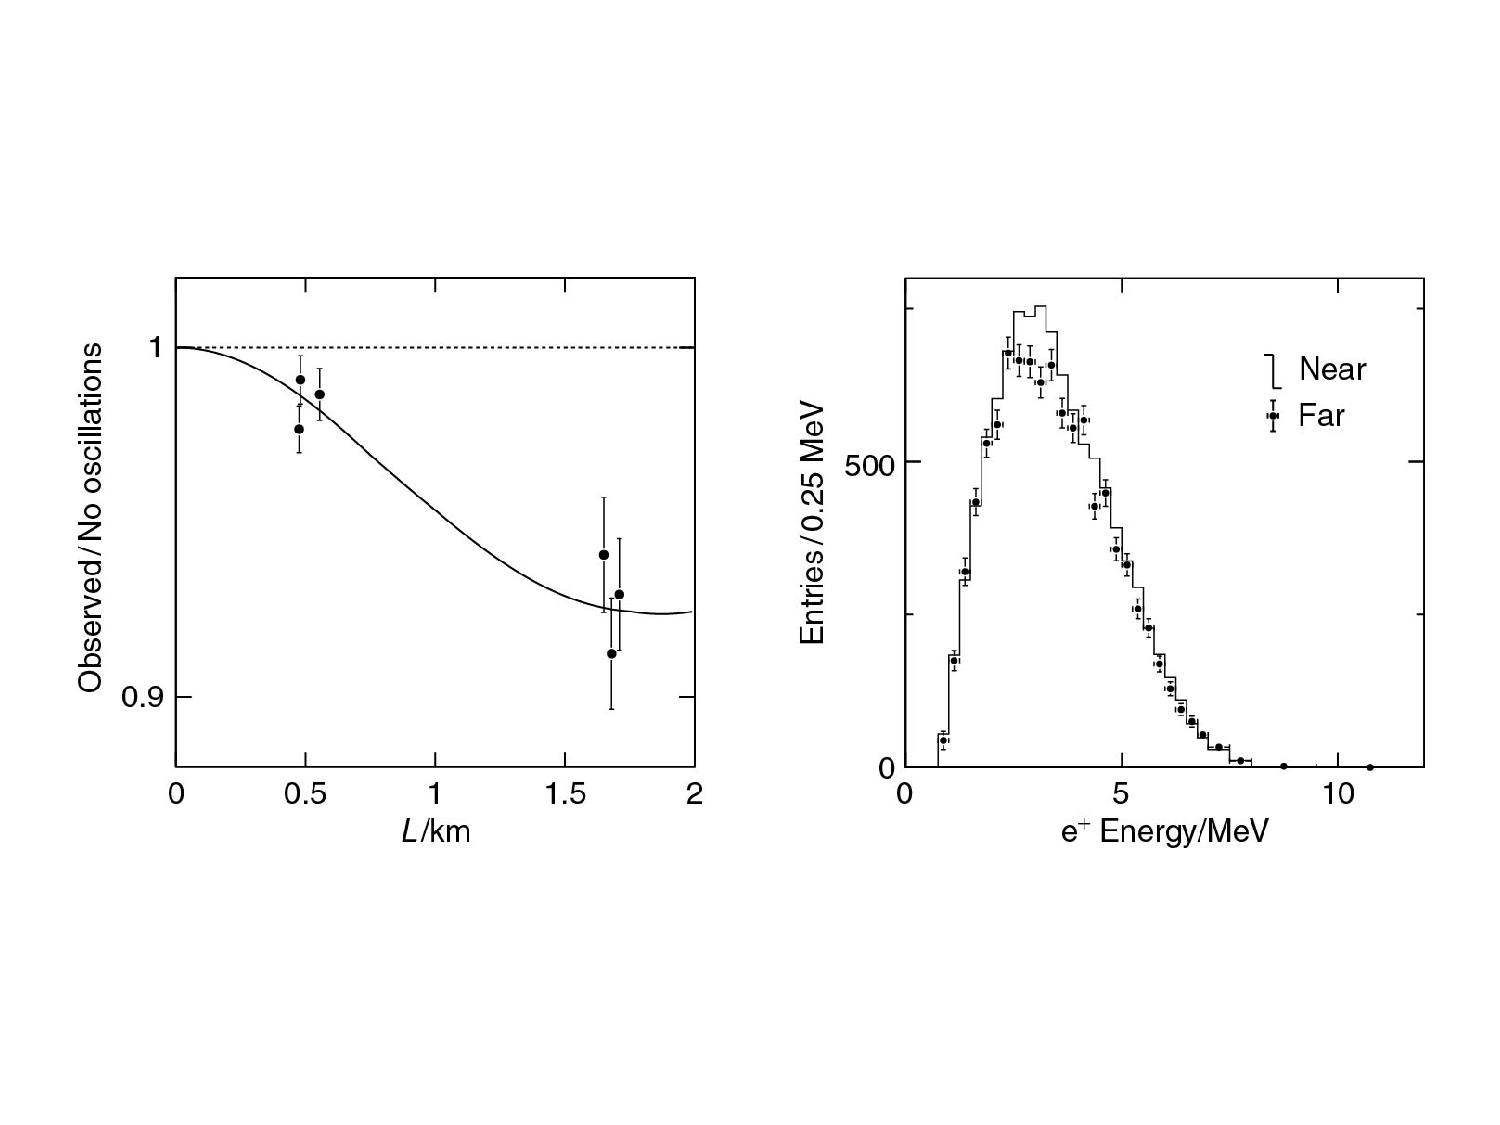
\includegraphics[width=0.85\textwidth,height=0.85\textheight,keepaspectratio]
                {pictures/t13_19.pdf}
  \vspace*{-20mm}
  \caption{Left: Daya Bay observed antineutrino rate compared to the
           unoscillated expectation (dotted line). Rates plotted as function
           of flux weighted distance to the reactors (solid line). Right:
           Daya Bay observed near and far e$^+$ energy spectra with the
           background subtracted. Image taken from Thomson Figure 13.19
           \cite{thomson_modern_2013}.}
\end{figure}

The Daya Bay experiment is an international reactor experiment based in China.
It consists of
six nuclear reactors and eight antineutrino detectors placed short, varied
distances (less than 2 km) away from the source. Hence the short
wavelength contribution of equation \eqref{eq:prb} dominates. Placing the
detectors at different distances allows cancellation of some systematic
uncertainty. The detectors are full of 20 tons of
liquid {\it scintillator}, a material that produces light when it interacts
with a particular particle but doesn't interfere with light itself.
The scintillator is doped with gadolinium and viewed by PMTs, which look for
the process \eqref{eq:betadecay}. Ascertaining whether such an event occurred
involves multiple steps. First the annihilation of the positron with an
electron produces two photons. The neutron scatters in the scintillator until
it is captured by a gadolinium nucleus, which takes roughly 100 $\mu$s and
produces photons. Photons from
the capture and the electron-positron annihilation yield Compton scattered
electrons, which then ionize the scintillator and produce scintillation light.
Hence the experiment counts an inverse beta decay event whenever it detects
a pulse of scintillation light followed by a neutron capture pulse
10-100~$\mu$s later.

\begin{figure}
  \centering
  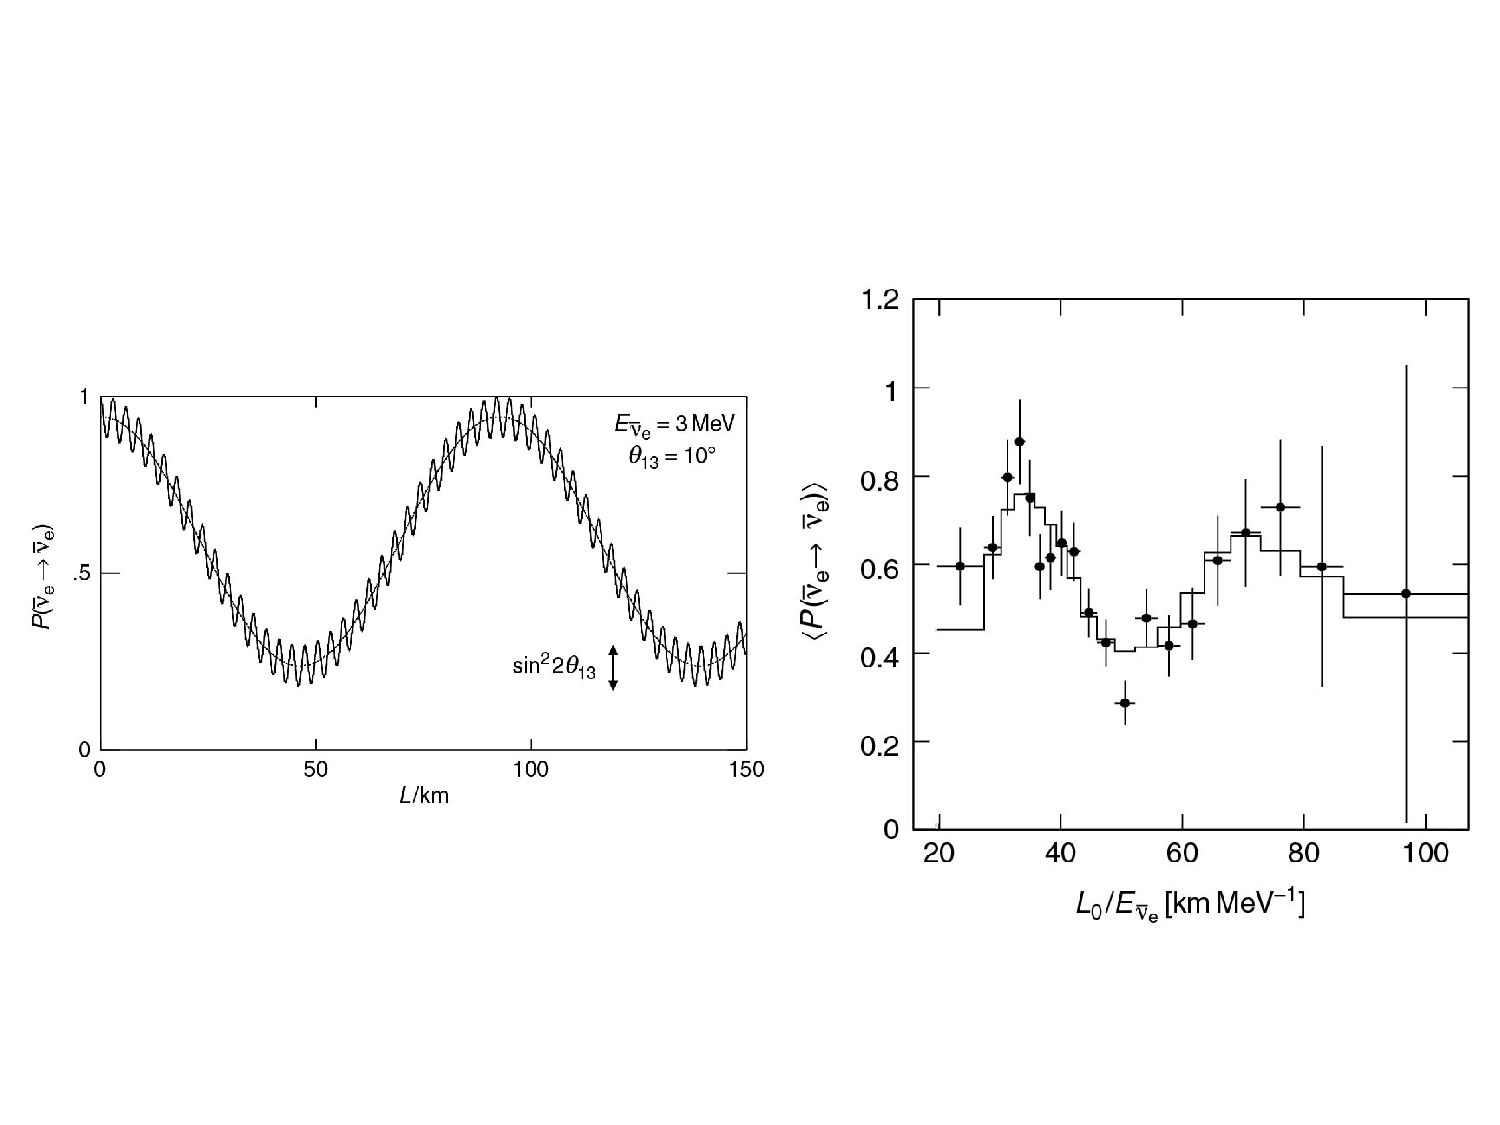
\includegraphics[width=0.90\textwidth,height=0.90\textheight,keepaspectratio]
                {pictures/t13_18&20.pdf}
  \vspace*{-10mm}
  \caption{Left: The electron antineutrino survival probability assuming
           $\theta_{12}=12$\textdegree, $\theta_{23}=45$\textdegree,
           $\theta_{13}=10$\textdegree, $\Delta m_{21}^2=8\times10^{-5}$
           $\text{eV}^2$, $\Delta m_{32}^2=2.5\time10^{-3}$ $\text{eV}^2$.
           Right: KamLAND data showing measured mean survival probability.
           The histogram is generated from the expected distribution given
           by the oscillation parameters that best fit the data, taking
           background into account. Images taken from Thomson Figures
           13.18 and 13.20 \cite{thomson_modern_2013}.}
\end{figure}

The results of the Daya Bay experiment are summarized in Figure 5. The left
plot compares the observed number of antineutrino events with the
unoscillated hypothesis. There is an unambiguous deviation
that increases with increasing detector distance.
The plot on the right compares the observed e$^+$ energy spectrum in the far
detectors to the spectrum of the near detectors, scaled to the same integrated
neutrino flux. Again the data are consistent with some electron neutrinos
oscillating to other flavors by the time they reach the far detector.
This energy difference then allows a measurement of $\theta_{13}$, and Daya Bay
found \cite{D1}
\begin{equation}
  \sin^2(2\theta_{13})=0.092\pm0.016(stat)\pm0.005(sys).
\end{equation}

The Kamioka Liquid Scintillator Antineutrino Detector (KamLAND) experiment,
located in the same mine as Super-K, consists of two concentric spheres in
water. The inner sphere is full of liquid scintillator and again surrounded by
PMTs, and neutrinos are detected using the same procedure as in Daya Bay.
However instead of gadolinium, the neutron capture occurs through the
process $\bar{\nu}_e+\text{p}\to\text{D}+\gamma$. The detector is situated
130-240 km away from the reactors, so that the long wavelength contribution of
\eqref{eq:prb} is the dominant term. The KamLAND data, depicted in the right
plot of Figure 6, form a rather nice pattern. The plot clearly shows electron
antineutrino survival probabilities that oscillate with $L_0/E_{\bar{\nu}e}$,
where $L_0$ is the flux weighted mean distance from the detector to the
reactors. By comparing this distribution with the long wavelength dominated
survival probability, KamLAND found \cite{K1}
\begin{equation}
  \Delta m_{12}^2=7.58^{+0.14}_{-0.13}(stat)
        \pm0.15(sys)\times10^{-5}~\text{eV}^2.
\end{equation}
KamLAND also determined
\begin{equation}
  \tan^2\theta_{12}=0.56^{+0.10}_{-0.07}(stat)^{+0.10}_{-0.06}(sys).
\end{equation}

\subsubsection{Accelerator Experiments}
Long baseline accelerator experiments typically have two detectors, one
situated near the source, which reveals the unoscillated neutrino energy
spectrum, and one far away, which reveals the oscillated spectrum.
Many systematic uncertainties cancel when both a near and far detector are
used.
An important accelerator experiment is the Main Injector Neutrino Oscillation
Search (MINOS) at Fermilab. The experiment measures oscillations
of a pure muon neutrino beam. It started collecting data in 2005 and
was recently upgraded to MINOS+ in 2013. The near detector is situated 1 km
from the source, while the far detector is located in a mine in Minnesota
735 km away. The detectors are made of iron plates with relatively
thin layers of
plastic scintillator. Scintillation light is passed from the scintillator to
PMTs using optical fibers, and the detector is magnetized to measure
muon momentum.

\begin{figure}
  \centering
  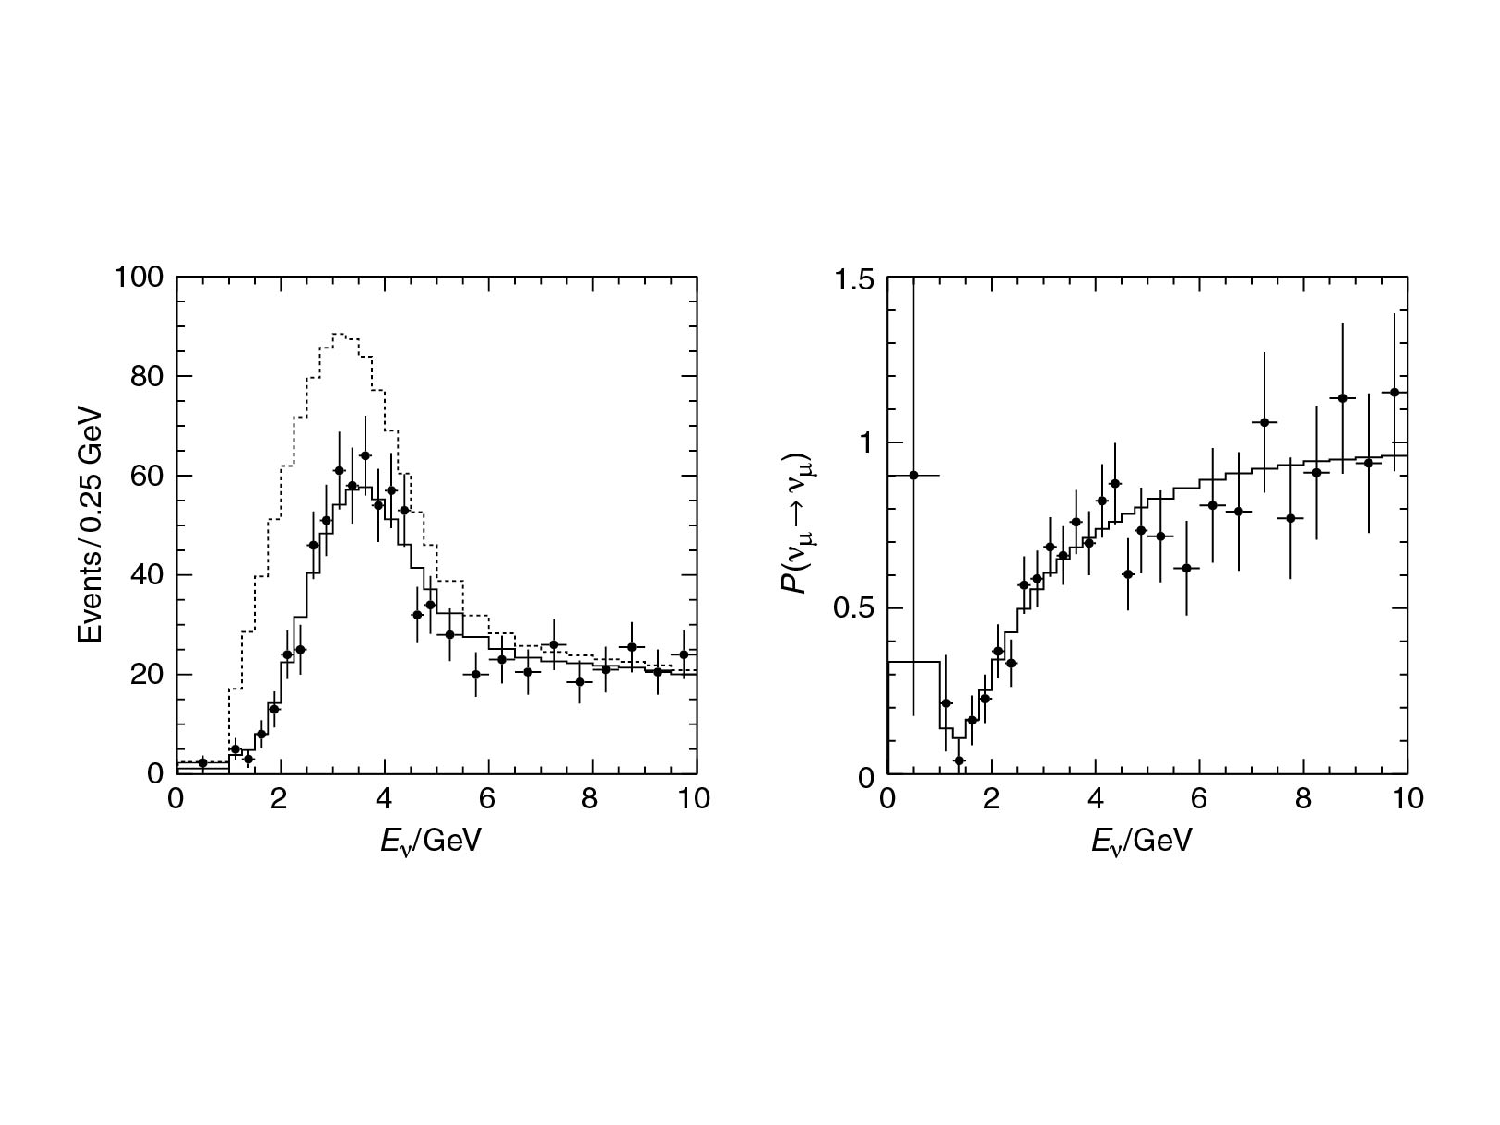
\includegraphics[width=0.90\textwidth,height=0.90\textheight,keepaspectratio]
                {pictures/t13_22.pdf}
  \vspace*{-20mm}
  \caption{Left: MINOS far detector energy spectrum and unoscillated
           prediction (dashed). Right: Muon neutrino survival probability
           as measured from the left figure. Image taken from Thomson
           Figure 13.22 \cite{thomson_modern_2013}.}
\end{figure}

We can calculate the general muon neutrino survival probability for MINOS
using the same arguments as the beginning of this subsection. We can write
\begin{equation}
  \label{eq:sexyprob}
  \begin{aligned}
    \pr{\nu_\mu\to\nu_\mu}
      &\approx 1-4|U_{\mu1}|^2|U_{\mu2}|^2\sin^2\Delta_{21}
              -4|U_{\mu3}|^2\left(1-|U_{\mu3}|^2\right)\sin^2\Delta_{32} \\
      &\approx 1-\left(\sin^2(2\theta_{23})c_{13}^4
                       +\sin^2(2\theta_{13})s_{23}^2)\right)
                        \sin^2\Delta_{32},
  \end{aligned}
\end{equation}
where in the last step we have utilized the fact that the long wavelength
component can be ignored for MINOS. Figure 7 shows the results of the
experiment. The left plot compares the observed far detector energy spectrum
with the unoscillated prediction, which gives a direct measurement of the
muon neutrino survival probability, shown on the right. According to equation
\eqref{eq:sexyprob}, the minimum of the right plot yields \cite{M1}
\begin{equation}
  |\Delta m_{32}^2|=(2.32^{+0.12}_{-0.08})\times10^{-3}~\text{eV}^2,
\end{equation}
and the best fit for $\theta_{23}$ yields the constraint
\begin{equation}
  \sin^2(2\theta_{23})\gtrsim0.90\
\end{equation}
at the 90\% confidence level.

\subsection{Conclusions, Outlook}
As has been demonstrated, the experimental evidence supporting the existence of
neutrino oscillations is very strong. The three flavor oscillation model seems
to predict the data quite well, and from the above experiments, we've (more or
less) determined the values of the parameters of the PMNS matrix.
The success of the model has been a triumph for particle
physicists, but there is still more we need to learn. For example we don't yet
know whether the neutrino is a Majorana spinor, which could shed light on the
viability of the seesaw mechanism. We also have not yet found the
phase $\delta$ of the PMNS matrix. The SM could accommodate another light
neutrino species. And of course there is still room to pin down the exact
value for $\theta_{23}$. The sheer number of neutrino experiments currently
performed and in progress, along with the most recent Nobel Prize, paints an
optimistic picture for the future of neutrino experiments; indeed, it is an
exciting time to be a neutrino physicist!

\bibliographystyle{unsrtnat}
\bibliography{bibliography}
